\documentclass[a4paper]{article}
\usepackage[utf8]{inputenc}
\usepackage[spanish, es-tabla]{babel}
\usepackage[table,xcdraw]{xcolor}
\usepackage{amsmath}
\usepackage{amsfonts}
\usepackage{amssymb}

\usepackage{float}
\usepackage{graphicx}

\usepackage{caption}
\usepackage{subcaption}
\captionsetup{compatibility=false}

\usepackage{multirow}
\setlength{\doublerulesep}{\arrayrulewidth}

\newcommand{\quotes}[1]{``#1''}
\newcommand\underrel[2]{\mathrel{\mathop{#2}\limits_{#1}}}

\usepackage{array}
\newcolumntype{C}[1]{>{\centering\let\newline\\\arraybackslash\hspace{0pt}}m{#1}}

\usepackage[american]{circuitikz}
\usepackage{xcolor}
\usepackage{fancyhdr}

\newlength{\stockheight}
\usepackage{hyperref}

\hypersetup{
    colorlinks=true,
    linkcolor=blue,
    filecolor=magenta,      
    urlcolor=blue,
    citecolor=blue,    
}

\urlstyle{same}

\usepackage{units} 
\pagestyle{fancy}
\fancyhf{}

\rfoot{Página \thepage}



\begin{document}
Es esta sección se implementará un SR-Latch y un Flip Flop D utilizando compuertas.
\subsection{SR-Latch}
Un Latch-SR es un elemento de memoria asincrónico, con dos inputs (S-R) también conocido con Set-Reset Latch. Le corresponde la siguiente tabla de verdad:

\begin{table}[H]
\centering
\begin{tabular}{
>{\columncolor[HTML]{FFFFFF}}c 
>{\columncolor[HTML]{FFFFFF}}c |
>{\columncolor[HTML]{FFFFFF}}c }
\textbf{$S$} & \textbf{$R$} & \textbf{$Q_n$} \\ \hline
0            & 0            & $Q_{n-1}$      \\
0            & 1            & 0              \\
1            & 0            & 1              \\
1            & 1            & 0             
\end{tabular}
\end{table}
El circuito propuesto de implementación es el siguiente:\footnote{Brown, S. and Vranesic, Z. (2002). Fundamentals of digital logic with VHDL design. 3rd ed. pp.250-251.}:
\begin{figure}[H]	
	\centering
	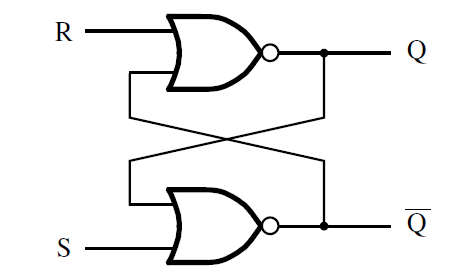
\includegraphics[width=0.5\textwidth]{Imagenes/srlatch.PNG}
	\caption{Circuito Propuesto SR-Latch.}
	\label{fig:circsrlatch}
\end{figure}
Se llevará a cabo utilizando compuertas NOR, se eligió el integrado 74HC02 debido a que es High-Speed y no es necesario compatibilidad con TTL, como se analizó en el punto (2). 

Se tomarán como observables  de interés el tiempo de propagación:
\begin{align} t_{p-SQ}: S \implies Q \ \ \ \textsuperscript{$\wedge$} \ \ \ t_{p-RQ}: R \implies Q \end{align} 

Estos tiempos serán comparados con un integrado 74HC279 el cual contiene 4 SR-Latch.
\subsection{Flip Flop D}
Un Flip Flop D es un elemento de memoria sincrónico,cuenta con  2 entradas siendo una de clock y la otra de la información (Data).Le corresponde la siguiente tabla de verdad:
% Please add the following required packages to your document preamble:
% \usepackage[table,xcdraw]{xcolor}
% If you use beamer only pass "xcolor=table" option, i.e. \documentclass[xcolor=table]{beamer}
\begin{table}[H]
\centering
\begin{tabular}{
>{\columncolor[HTML]{FFFFFF}}c 
>{\columncolor[HTML]{FFFFFF}}c |
>{\columncolor[HTML]{FFFFFF}}c }
\textbf{Clock} & \textbf{$D$} & \textbf{$Q_n$} \\ \hline
$\downarrow$   & X            & $Q_{n-1}$      \\
$\uparrow$     & 0            & 0              \\
$\uparrow$     & 1            & 1             
\end{tabular}
\end{table}
El circuito propuesto de implementación es el siguiente:\footnote{Brown, S. and Vranesic, Z. (2002). Fundamentals of digital logic with VHDL design. 3rd ed. pp.254-256.}:
\begin{figure}[H]	
	\centering
	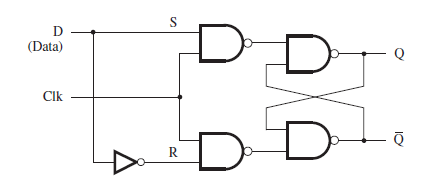
\includegraphics[width=0.8\textwidth]{Imagenes/dff.PNG}
	\caption{Circuito Propuesto Flip Flop D.}
	\label{fig:circsrlatch}
\end{figure}
Se llevará a cabo utilizando compuertas NAND, se eligió el integrado 74HC132  debido a que es High-Speed y no es necesario compatibilidad con TTL, como se analizó en el punto (2). 

Se tomarán como observables  de interés el tiempo de propagación:
\begin{align} t_{p-SQ}: D \implies Q \end{align} 

Estos tiempos serán comparados con un integrado 74HC374 el cual contiene 8 Flip Flop D.

\end{document}
